\documentclass{article}
\usepackage[utf8]{inputenc} %кодировка
\usepackage[T2A]{fontenc}
\usepackage[english,russian]{babel} %русификатор 
\usepackage{mathtools} %библиотека матеши
\usepackage[left=1cm,right=1cm,top=2cm,bottom=2cm,bindingoffset=0cm]{geometry} %изменение отступов на листе
\usepackage{amsmath}
\usepackage{graphicx} %библиотека для графики и картинок
\graphicspath{}
\DeclareGraphicsExtensions{.pdf,.png,.jpg}
\usepackage{subcaption}
\usepackage{pgfplots}
\usepackage{float}
\usepackage{listings}           
\lstset{
    language=Java,
    breaklines=true,
}

\begin{document}
% НАЧАЛО ТИТУЛЬНОГО ЛИСТА
\begin{center}
    \Large
    Федеральное государственное автономное \\
    образовательное учреждение высшего образования \\ 
    «Научно-образовательная корпорация ИТМО»\\
    \vspace{0.5cm}
    \large
    Факультет программной инженерии и компьютерной техники \\
    Направление подготовки 09.03.04 Программная инженерия \\
    \vspace{1cm}
    \Large
    \textbf{Отчёт по лабораторной работе №1} \\
        По дисциплине «Бизнес логика программных систем» ( семестр 7)\\
    \large
    \vspace{8cm}

    \begin{minipage}{.33\textwidth}
    \end{minipage}
    \hfill
    \begin{minipage}{.4\textwidth}
    
        \textbf{Студент}: \vspace{.1cm} \\
        \ Дениченко Александр P3312\\
        \textbf{Практик}:  \\
        \ Бобрусь Александр
    \end{minipage}
    \vfill
Санкт-Петербург\\ 2025 г.
\end{center}
\pagestyle{empty}
% КОНЕЦ ТИТУЛЬНОГО ЛИСТА 
\newpage
\pagestyle{plain}

\section*{Данные}


Переработать программу, созданную в результате выполнения лабораторной работы \#3, следующим образом:

Для управления бизнес-процессом использовать BPM-движок Camunda.
Заменить всю "статическую" бизнес-логику на "динамическую" на базе BPMS. Весь бизнес-процесс, реализованный в ходе выполнения предыдущих лабораторных работ (включая разграничение доступа по ролям, управление транзакциями, асинхронную обработку и периодические задачи), должен быть сохранён!.
BPM-движок должен быть встроен в веб-приложение (embedded mode).
Для описания бизнес-процесса необходимо использовать приложение Camunda Modeler.
Пользовательский интерфейс приложения должен быть сгенерирован с помощью генератора форм Camunda.
Итоговая сборка должно быть развёрнута на сервере helios под управление сервера приложений WildFly.
Правила выполнения работы:

Описание бизнес-процесса необходимо реализовать на языке BPMN 2.0.
Необходимо интегрировать в состав процесса, управляемого BPMS, всё, что в принципе возможно в него интегрировать. Если какой-то из компонентов архитектуры приложения (например, асинхронный обмен сообщениями с помощью JMS) не поддерживается, необходимо использовать для интеграции с этой подсистемой соответствующие API и адаптеры.
Распределённую обработку задач и распределённые транзакции на BPM-движок переносить не требуется.
\section*{Выполнение}

\begin{center}
    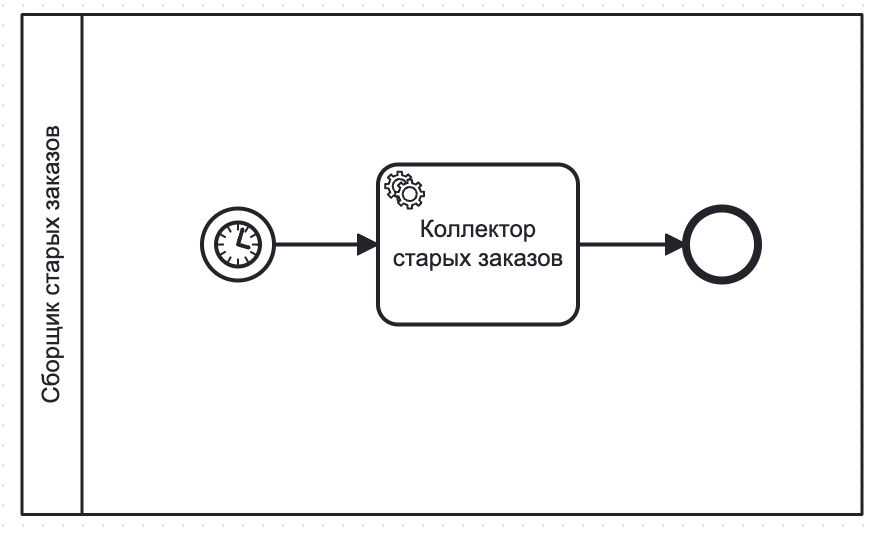
\includegraphics[width=.9\textwidth]{collector.png}
\end{center}

\begin{center}
    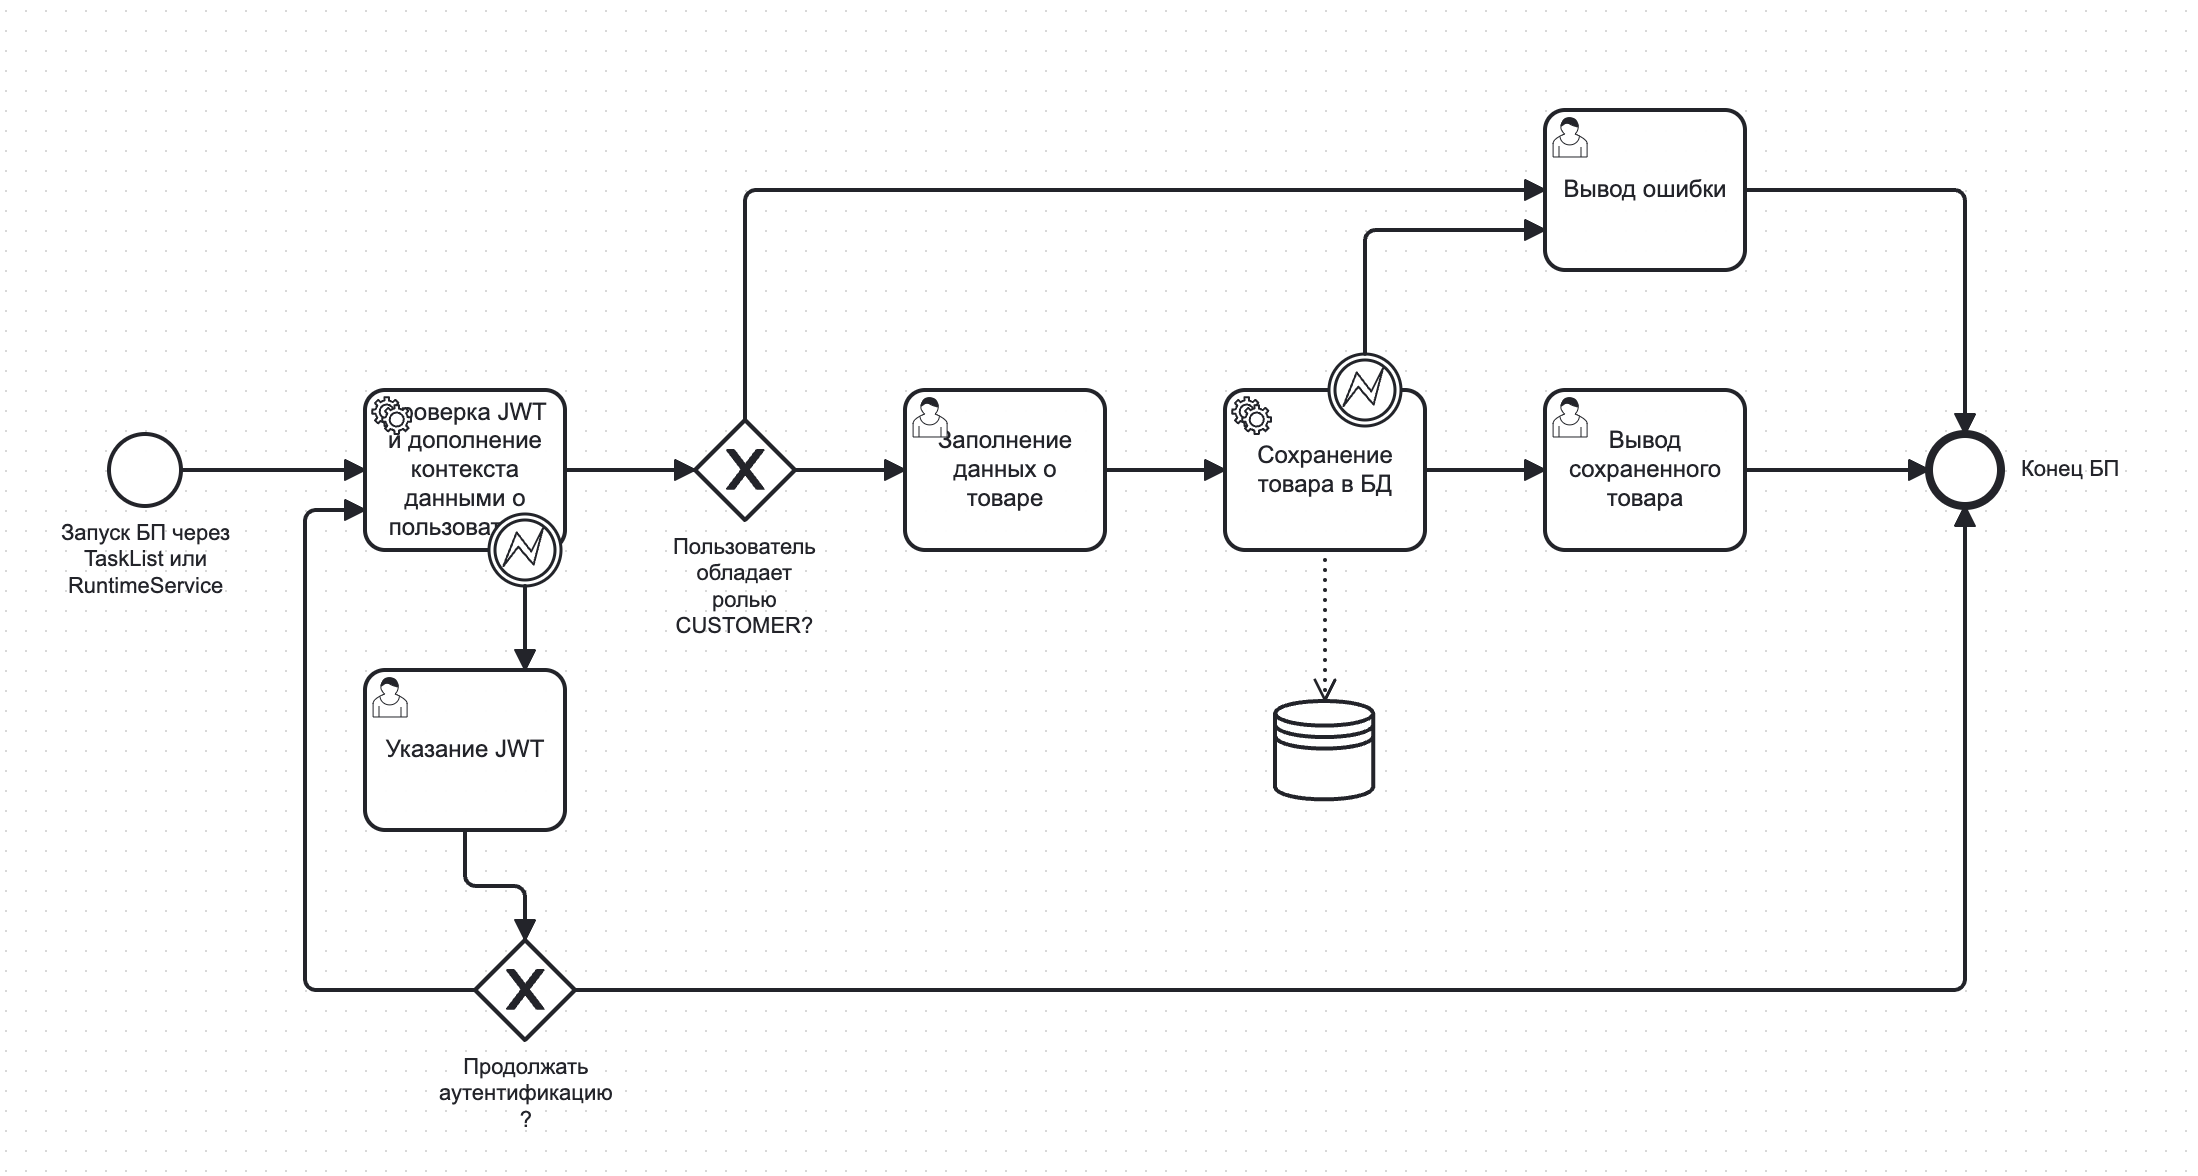
\includegraphics[width=.9\textwidth]{1.png}
\end{center}

\begin{center}
    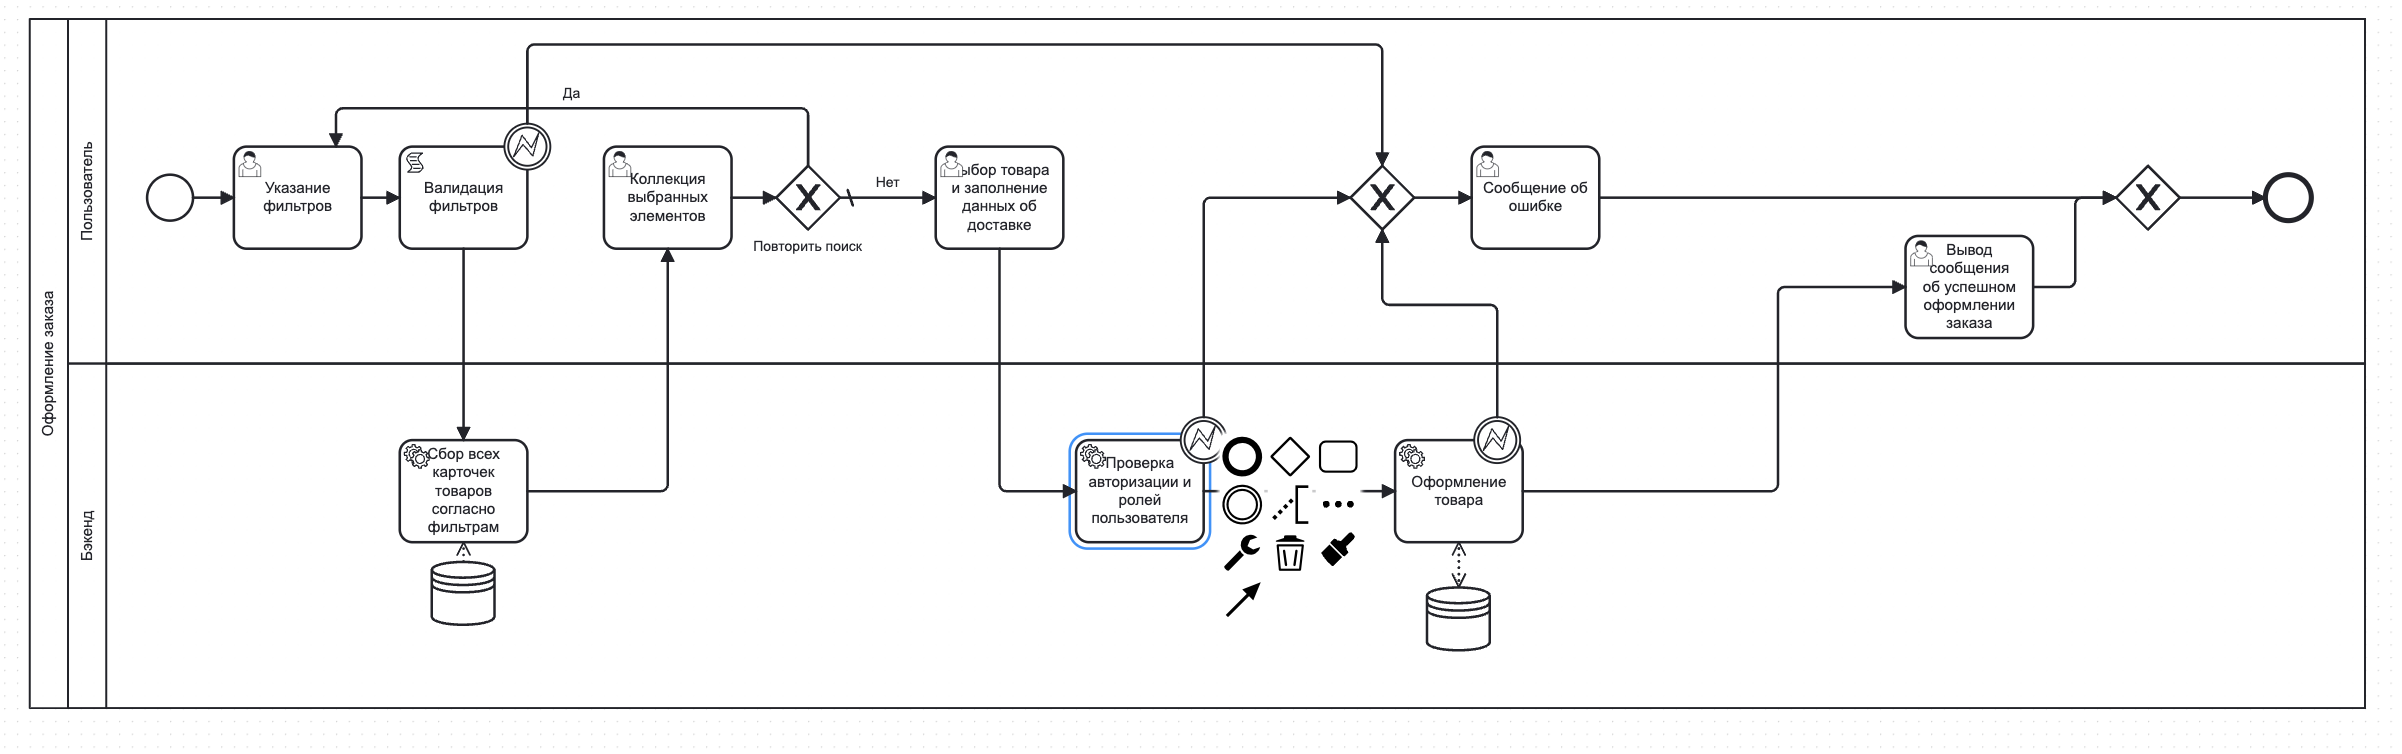
\includegraphics[width=.9\textwidth]{2.png}
\end{center}

\begin{center}
    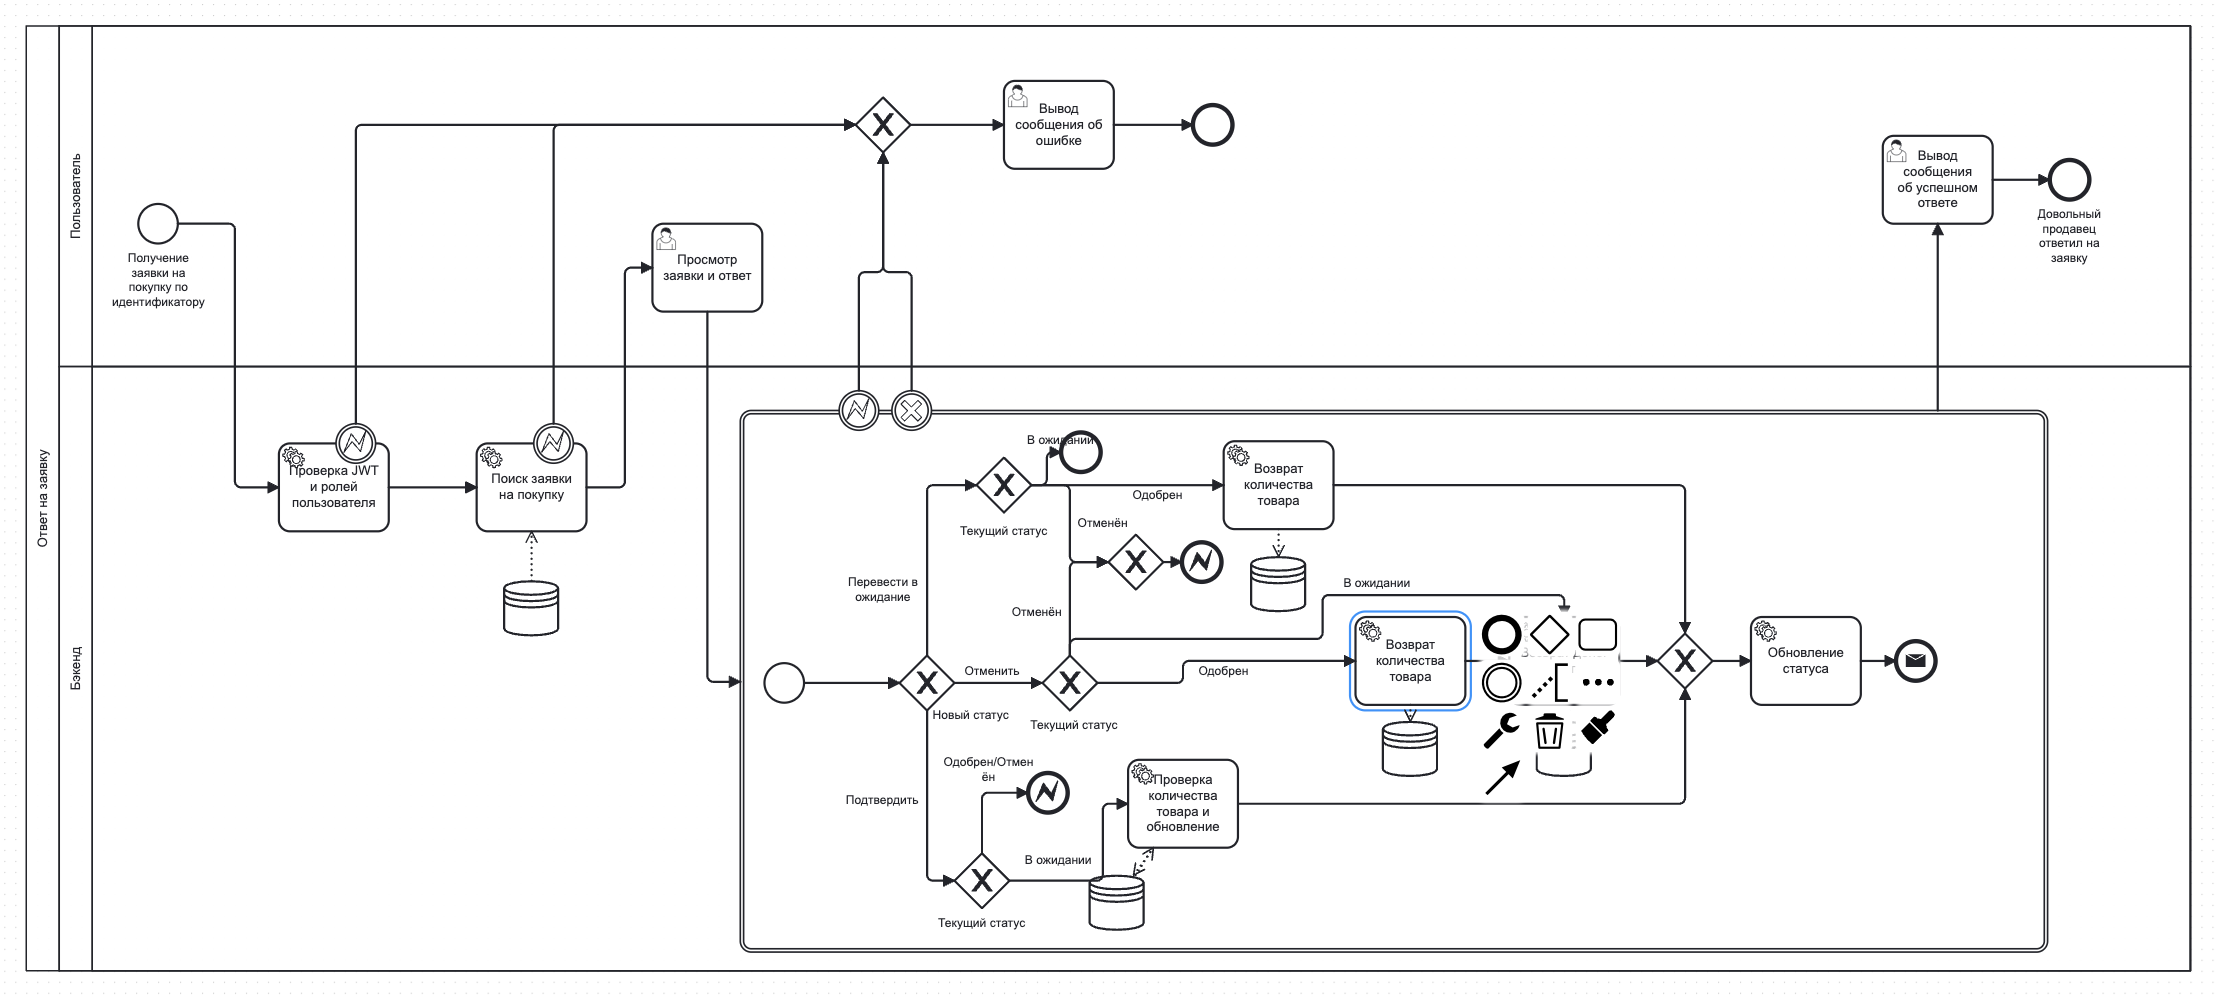
\includegraphics[width=.9\textwidth]{3.png}
\end{center}

Делегаторы
\begin{lstlisting}[language=Java]
@Component
@Slf4j
@RequiredArgsConstructor
public class CollectorDelegator implements JavaDelegate {

    private final OrderService orderService;

    @Override
    public void execute(DelegateExecution execution) throws Exception {
        log.info("================ COLLECTOR JOB STARTED at {} ================", LocalDateTime.now());
        try {
            orderService.clearOlderThan(LocalDateTime.now().minusDays(3));
            log.info("Orders older than 3 days have been cleared successfully");
        } catch (Exception e) {
            log.error("Error while executing CollectorJob: {}", e.getMessage(), e);
        }
        log.info("================ COLLECTOR JOB FINISHED at {} ================", LocalDateTime.now());
    }
}
\end{lstlisting}
\begin{lstlisting}[language=Java]

@Component
@RequiredArgsConstructor
@Slf4j
public class WorkerOrderNotification {
    private final OrderRepository orderRepository;
    private final CustomMessageProducer messageProducer;

    @Value("${camunda.bpm.client.base-url}")
    private String camundaBaseUrl;

    private final String WORKER_ID = "orderNotificationWorker";
    private final String TOPIC_NAME = "send-order-notification";
    private final long LOCK_DURATION_MS = 10000L;

    @PostConstruct
    public void subscribe() {
        ExternalTaskClient client = ExternalTaskClient.create()
                .baseUrl(camundaBaseUrl)
                .workerId(WORKER_ID)
                .asyncResponseTimeout(20000)
                .build();


        TopicSubscriptionBuilder subscriptionBuilder = client.subscribe(TOPIC_NAME)
                .lockDuration(LOCK_DURATION_MS)
                .handler((externalTask, externalTaskService) -> {
                    String businessKey = externalTask.getBusinessKey();
                                externalTask.getId(), TOPIC_NAME, businessKey);

                    try {
                        
                        Long orderId = (long) externalTask.getVariable("order_id");
                        Order order = orderRepository.findById(orderId).orElseThrow(() -> new RuntimeException("Order not found"));

                        final OrderMessageDto orderMessageDto = OrderMapper.toMessageDto(order);
                        
                        messageProducer.sendOrderMessage(orderMessageDto);

                        externalTaskService.complete(externalTask);

                    } catch (Exception e) {
                        
                            externalTaskService.handleBpmnError(
                                externalTask,
                                "NOTIFICATION_ERROR"                            );
                        
                    }
                });

        subscriptionBuilder.open();
    }
}    
\end{lstlisting}

\begin{lstlisting}
@Component
@RequiredArgsConstructor
public class CheckAndUpdateOrderDelegator implements JavaDelegate {
    private final ProductRepository productRepository;

    @Override
    public void execute(DelegateExecution execution) throws Exception {
        Long productId = (Long) execution.getVariable("product_id");
        Product product = productRepository.findById(productId).get();

        if(product.getQuantity() < (int) (long) execution.getVariable("quantity")) {
            execution.setVariable("error");
            throw new BpmnError("NOT_ENOUGH_PRODUCTS");
        }else{
            product.setQuantity(product.getQuantity() - (int) (long) execution.getVariable("quantity"));
        }
        productRepository.save(product);
    }
}
\end{lstlisting}

\begin{lstlisting}
@Component
@RequiredArgsConstructor
public class CreateOrderDelegator implements JavaDelegate {

    private static final Logger log = LoggerFactory.getLogger(CreateOrderDelegator.class);

    private final OrderService orderService;
    private final JwtUtils jwtUtils;
    private final UserRepository userRepository;

    @Override
    public void execute(DelegateExecution execution) throws Exception {
        String token = (String) execution.getVariable("token");

        try {
            if (token == null || !jwtUtils.validateJwtToken(token)) {
                log.error("Invalid or missing token for process instance {}", execution.getProcessInstanceId());
                throw new BpmnError("INVALID_TOKEN", "Authentication token is invalid or missing.");
            }

            String username = jwtUtils.getUsernameFromJwtToken(token);

            User user = userRepository.findByEmail(username)
                    .orElseThrow(() -> {
                        log.error("User not found for username {} from token", username);
                        return new BpmnError("USER_NOT_FOUND", "User details not found for token.");
                    });

            UserDetails userDetails = UserDetailsImpl.build(user);

            UsernamePasswordAuthenticationToken authentication = new UsernamePasswordAuthenticationToken(
                    userDetails,
                    null,
                    userDetails.getAuthorities()
            );

            SecurityContextHolder.getContext().setAuthentication(authentication);
            log.info("User '{}' manually authenticated for order creation.", username);

            boolean hasRequiredRole = userDetails.getAuthorities().stream()
                    .anyMatch(grantedAuthority -> grantedAuthority.getAuthority().equals("ORDER_CREATE"));

            if (!hasRequiredRole) {
                log.warn("User '{}' does not have required role for order creation.", username);
                throw new BpmnError("NO_REQUIRED_ROLE", "User does not have required role to create order.");
            }

            String productIdsString = (String) execution.getVariable("products");
            HashMap<Long, Integer> productsMap = parseProductString(productIdsString);

            String city = (String) execution.getVariable("city");
            String street = (String) execution.getVariable("street");

            if (city == null || street == null) {
                throw new BpmnError("MISSING_ADDRESS_INFO", "City or street information is missing.");
            }
            if (productsMap.isEmpty()) {
                throw new BpmnError("EMPTY_PRODUCT_LIST", "Cannot create an order with no valid products.");
            }

            log.info("Calling orderService.create for user '{}'", username);
            orderService.create(CreateOrderDto.builder()
                .city(city)
                .street(street)
                .products(productsMap)
                .build());

            log.info("Order created successfully with products: {}", productsMap);

        } finally {
            SecurityContextHolder.clearContext();
            log.debug("SecurityContext cleared after order creation delegate.");
        }
    }

    private HashMap<Long, Integer> parseProductString(String productIdsString) {
        HashMap<Long, Integer> productsMap = new HashMap<>();
        if (productIdsString != null && !productIdsString.trim().isEmpty()) {
            String[] productIds = productIdsString.split(",");
            for (String idStr : productIds) {
                try {
                    String[] parts = idStr.trim().split("-");
                    Long productId = Long.parseLong(parts[0]);
                    int quantity = Integer.parseInt(parts[1]);
                    productsMap.put(productId, quantity);
                } catch (NumberFormatException e) {
                    log.error("Could not parse product ID: {}", idStr.trim(), e);
                    throw new BpmnError("INVALID_PRODUCT_ID_FORMAT", "Invalid product ID format: " + idStr.trim());
                }
            }
        } else {
            log.warn("Product variable string is empty or null.");
        }
        return productsMap;
    }
}
\end{lstlisting}

\begin{lstlisting}
@
@Component
@RequiredArgsConstructor
public class OrderFinder implements JavaDelegate {

    private final OrderRepository orderRepository;

    private final UserRepository userRepository;

    @Override
    public void execute(DelegateExecution delegateExecution) throws Exception {
        long orderId = (long) delegateExecution.getVariable("order_id");

        Order order = orderRepository.findById(orderId)
                .orElseThrow(() -> {
                    delegateExecution.setVariable("error", "order not found");
                    return new BpmnError("order not found");
                });

        User user = userRepository.findByEmail((String) delegateExecution.getVariable("user_email"))
                .orElseThrow(() -> {
                    delegateExecution.setVariable("error", "user not found");
                    return new BpmnError("User not found");
                });

       if (!(boolean) delegateExecution.getVariable("hasRoleCustomer")) {
           delegateExecution.setVariable("error", "user is not a customer");
           throw new BpmnError("user is not a customer");
       }

       if (order.getCustomer().getId() != user.getId()) {
           delegateExecution.setVariable("error", "order is not assigned to customer");
           throw new BpmnError("order is not assigned to customer");
       }

       delegateExecution.setVariable("city", order.getCity());
       delegateExecution.setVariable("quantity", order.getQuantity());
       delegateExecution.setVariable("name", order.getProduct().getName());
       delegateExecution.setVariable("status", order.getStatus().name());
       delegateExecution.setVariable("product_id", order.getProduct().getId());
       delegateExecution.setVariable("cost", order.getProduct().getPrice() * order.getQuantity());

    }
}
\end{lstlisting}

\begin{lstlisting}
@Component
@RequiredArgsConstructor
public class StatusUpdateDelegator implements JavaDelegate {

    private final OrderRepository orderRepository;

    @Override
    public void execute(DelegateExecution execution) throws Exception {
        Long orderId = (Long) execution.getVariable("order_id");
        Order order = orderRepository.findById(orderId).get();
        order.setStatus(OrderStatus.valueOf((String) execution.getVariable("answer")));
        orderRepository.save(order);
    }
}
\end{lstlisting}

\begin{lstlisting}
    @Component
@RequiredArgsConstructor
public class JwtChecker implements JavaDelegate {

    private final JwtUtils jwtUtils;
    private final UserRepository userRepository;

    @Override
    public void execute(DelegateExecution delegateExecution) throws Exception {
        String token = (String) delegateExecution.getVariable("token");
        if (token == null) {
            delegateExecution.setVariable("error", "token is null");
            throw new BpmnError("token is null");
        }
        if (!jwtUtils.validateJwtToken(token)) {
            delegateExecution.setVariable("error", "token is invalid");
            throw new BpmnError("invalid token");
        }

        User user = userRepository.findByEmail(jwtUtils.getUsernameFromJwtToken(token))
                .orElseThrow(() -> {
                    delegateExecution.setVariable("error", "user not found");
                    return new BpmnError("user not found");
                });
        delegateExecution.setVariable("user_email", user.getEmail());

        boolean hasRoleCustomer = false;
        boolean hasRoleUser = false;
        boolean hasRoleAdmin = false;
        for (Role role : user.getRoles()) {
            if (role.getName() == RoleEnum.ROLE_CUSTOMER)
                hasRoleCustomer = true;
            if (role.getName() == RoleEnum.ROLE_USER)
                hasRoleUser = true;
            if (role.getName() == RoleEnum.ROLE_ADMIN)
                hasRoleAdmin = true;
        }
        delegateExecution.setVariable("hasRoleCustomer", hasRoleCustomer);
        delegateExecution.setVariable("hasRoleUser", hasRoleUser);
        delegateExecution.setVariable("hasRoleAdmin", hasRoleAdmin);
        System.out.println(hasRoleCustomer);
    }

}
\end{lstlisting}



\begin{lstlisting}
@Component
@RequiredArgsConstructor
public class ProductSaver implements JavaDelegate {

    private final ProductRepository productRepository;
    private final UserRepository userRepository;

    @Override
    public void execute(DelegateExecution delegateExecution) throws Exception {
        String name = (String) delegateExecution.getVariable("product_name");
        String description = (String) delegateExecution.getVariable("product_description");
        double price = ((double) (long) delegateExecution.getVariable("product_price")) / 100;
        ProductType productType = ProductType.valueOf(delegateExecution.getVariable("product_type").toString());
        int quantity = (int) (long) delegateExecution.getVariable("product_quantity");

        User user = userRepository.findByEmail((String) delegateExecution.getVariable("user_email"))
                .orElseThrow(() -> new BpmnError(""));
        Product product = new Product(0, name, description, price, quantity, productType, user);
        try {
            product = productRepository.save(product);
        } catch (Exception e) {
            throw new BpmnError("");
        }
        delegateExecution.setVariable("product_id", product.getId());
    }
}
\end{lstlisting}

\begin{lstlisting}  

@Component
@RequiredArgsConstructor
public class ReturnMoneyDelegator implements JavaDelegate { 
    private final UserRepository userRepository;

    @Override
    public void execute(DelegateExecution execution) throws Exception {
        String email = (String) execution.getVariable("user_email");
        User user = userRepository.findByEmail(email).get();
        user.setBalance(user.getBalance() + (double) execution.getVariable("cost"));
        userRepository.save(user);
    }
}
\end{lstlisting}

\section*{Вывод}

Изучено использование BPM-движка Camunda для управления бизнес-процессами.



\end{document}
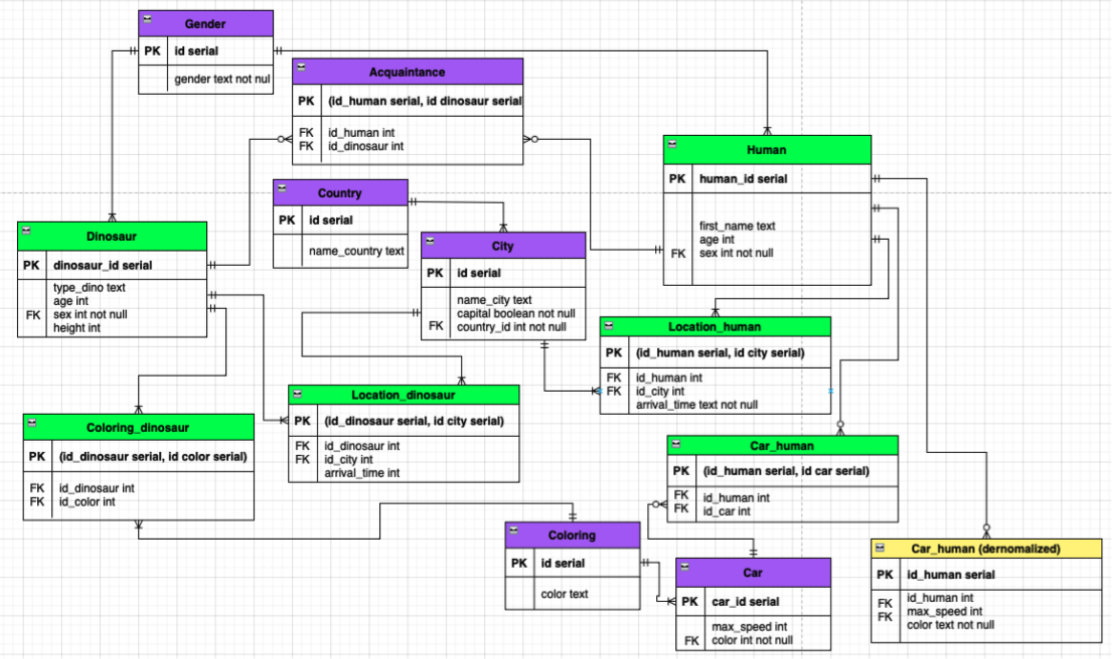
\includegraphics[width=.9\textwidth]{123}